\section{Versuchsaufbau/-durchführung}
Für die verschiedenen Versuchsaufbauten werden die folgenden Bauelemente
\begin{align}
\begin{aligned}
  L&=\SI{1,75}{\milli\henry}\\
  C_1&=\SI{22,0}{\nano\farad}\\
  C_2&=\SI{9,39}{\nano\farad}
\end{aligned}
\end{align}
verwendet.

\subsection{Bestimmung der Durchlasskurve für den $LC$- und $LC_1 C_2$ Kette}
Zunächst wird der Versuch, nach Abbildung \ref{fig:aufbau_durchlass} aufgebaut. %überarbeite diesen satz nochmal
\begin{figure}
  \centering
  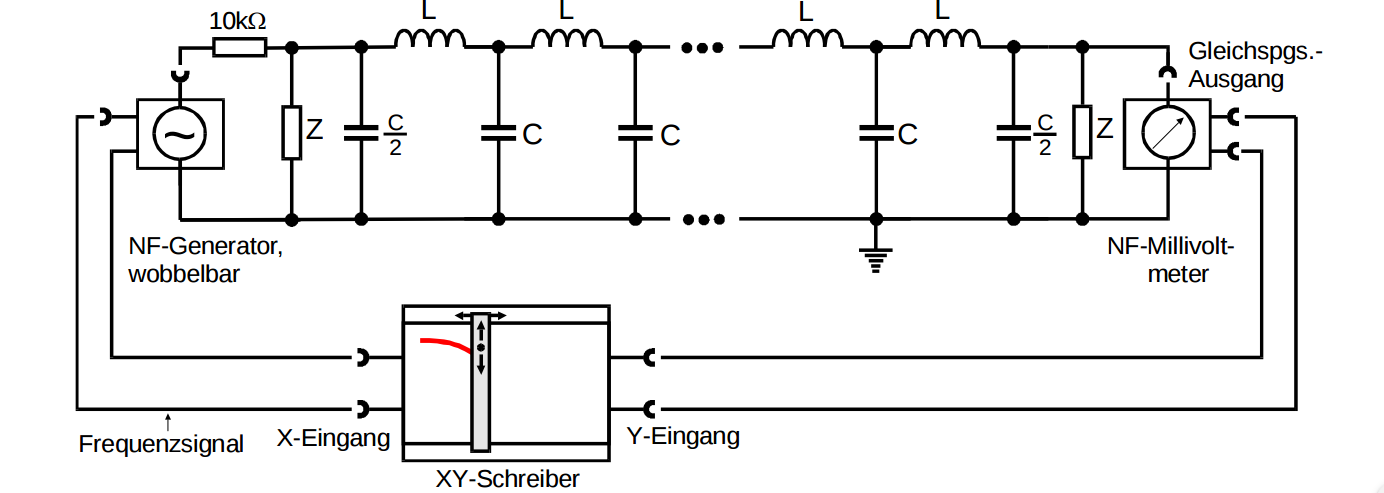
\includegraphics[width=0.8\textwidth]{bilder/versuchsaufbau_1.png}
  \caption{Versuchsaufbau für die Bestimmung der Durchlasskurve.\cite{anleitung356}}
  \label{fig:aufbau_durchlass}
\end{figure}

Zu Beginn wird an dem NF-Generator ein Frequenz Sweep eingestellt.
In dem Frequenzbereich des Sweeps muss die Grenzfrequenz liegen, bei der die
Kettenschaltung stromundurchlässig wird. %stromundurchlässig
Am Kettenanfang und -ende werden die Widerstände $Z$ auf den theoretisch
berechneten Wellenwiderstand eingestellt.
Die am Kettenende anliegende Spannung und die vom Generator ausgegebenen Frequenzen
werden an einem XY-Schreiber gegeneinander aufgetragen.
Wichtig dabei ist, dass zu beliebig ausgewählten Punkten, die gerade anliegende Frequenz bekannt ist.
Deshalb werden für 6 Referenzpunkte die Spannung notiert.  %Hier noch mehr dazu ? %sag einfach, dass 6 referenzpunkte aufgenommen wurden

\subsection{Bestimmung der Dispersionskurve}
Der Versuch wird, wie in Abbildung \ref{fig:aufbau_dispersion} zu sehen ist, aufgebaut.%überarbeite diesen satz nochmal
\begin{figure}
  \centering
  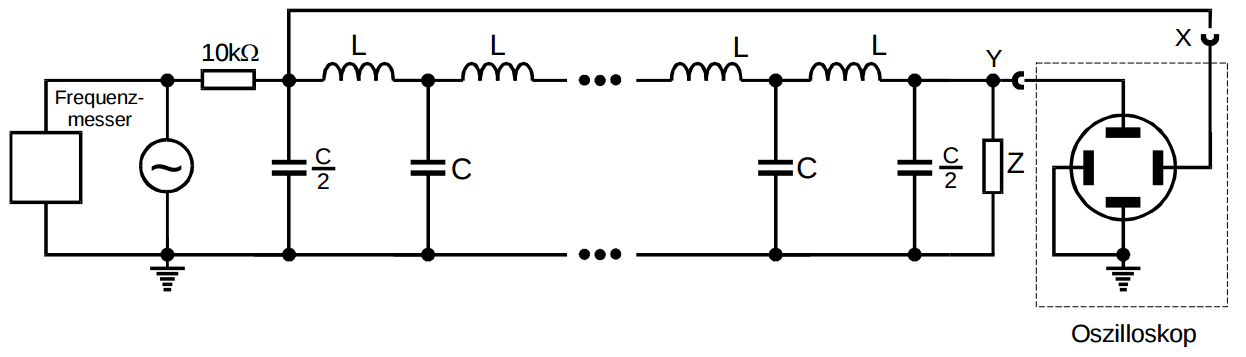
\includegraphics[width=0.8\textwidth]{bilder/versuchsaufbau_dispersion.png}
  \caption{Versuchsaufbau für die Messung der Dispersionskurve.\cite{anleitung356}}
  \label{fig:aufbau_dispersion}
\end{figure}
Anschließend werden für die verwendeten Bauteile
die Wellenwiderstände berechnet %für die verwendeten Bauteile
und die An- und Abschlusswiderstände $Z$ auf diesen Wert eingestellt.
Mithilfe von Lissajous-Figuren werden nun die Frequenzen bestimmt, die eine Phasenverschiebung von $n\pi$ %'wo' umgangssprachlich
hervor rufen. Anschließend kann dann mit der Anzahl der Kettenglieder auf die %-komma
Phasenverschiebung pro Kettenglied geschlossen werden.

\subsection{Ausmessung der stehende Welle}
Der Versuch wird nach Abb. \ref{fig:aufbau_dispersion} aufgebaut.
Nun wird mit und ohne Wellenwiederstand $Z$, die Spannung mit einem Millivoltmeter gemessen. %überarbeite diesen satz nochmal
Zunächst wird die Spannung am Kettenanfang abgegriffen, um so ein frequenzabhängiges Spannungsmaximum
zu finden. Für die ersten beiden Maxima werden bei allen Kettengliedern die anliegende Spannung gemessen. % zu finden
Für die restlichen Maxima werden nur die dazugehörigen Frequenzen notiert.
